\documentclass[twoside,11pt]{article}

% Any additional packages needed should be included after jmlr2e.
% Note that jmlr2e.sty includes epsfig, amssymb, natbib and graphicx,
% and defines many common macros, such as 'proof' and 'example'.
%
% It also sets the bibliographystyle to plainnat; for more information on
% natbib citation styles, see the natbib documentation, a copy of which
% is archived at http://www.jmlr.org/format/natbib.pdf

\usepackage{jmlr2e}
\usepackage{enumitem}
\usepackage[utf8]{inputenc}  %% Support French accents
\usepackage{booktabs}        %% Good looking tables
\usepackage{pifont}          %% http://ctan.org/pkg/pifont
\usepackage{xspace}
\usepackage{xcolor}
\usepackage{threeparttable}  %% Footnotes in tables
\usepackage{lastpage}

% Definitions of handy macros can go here
\newcommand{\dataset}{{\cal D}}
\newcommand{\fracpartial}[2]{\frac{\partial #1}{\partial  #2}}
\newcommand{\skmultiflow}{\textsf{scikit-multiflow}\xspace}
\newcommand{\sklearn}{\textsf{scikit-learn}\xspace}
\newcommand{\weka}{\textsf{WEKA}\xspace}
\newcommand{\moa}{\textsf{MOA}\xspace}
\newcommand{\meka}{\textsf{MEKA}\xspace}
\newcommand{\streammodel}{\textsf{StreamModel}\xspace}
\newcommand{\streamevaluator}{\textsf{StreamEvaluator}\xspace}
\newcommand{\stream}{\textsf{Stream}\xspace}
\newcommand{\reffig}[1]{Figure~\ref{#1}}
\newcommand{\reftab}[1]{Table~\ref{#1}}
\newcommand{\refsec}[1]{Sec.~\ref{#1}}
\newcommand{\cmark}{\ding{51}}  % check mark
\newcommand{\xmark}{\ding{55}}  % cross mark

% Heading arguments are {volume}{year}{pages}{submitted}{published}{author-full-names}

\jmlrheading{19}{2018}{1-\pageref{LastPage}}{4/18}{10/18}{18-251}{Jacob Montiel and Jesse Read and Albert Bifet and Talel Abdessalem}

% Short headings should be running head and authors last names

\ShortHeadings{
Scikit-Multiflow: A Multi-output Streaming Framework
}{Montiel and Read and Bifet and Abdessalem}
\firstpageno{1}

\begin{document}

\title{
Scikit-Multiflow: A Multi-output Streaming Framework
}

\author{\name Jacob Montiel \email jacob.montiel@telecom-paristech.fr \\
       \addr LTCI,
       Télécom ParisTech, Université Paris-Saclay\\
       Paris, FRANCE
       \AND
       \name Jesse Read \email jesse.read@polytechnique.edu \\
       \addr LIX, 
       École Polytechnique\\
       Palaiseau, FRANCE
       \AND
       \name Albert Bifet \email albert.bifet@telecom-paristech.fr \\
       \addr LTCI,
       Télécom ParisTech, Université Paris-Saclay\\
       Paris, FRANCE
       \AND
       \name Talel Abdessalem \email talel.abdessalem@enst.fr \\
       \addr LTCI, 
       Télécom ParisTech, Université Paris-Saclay\\
       Paris, FRANCE \\
       UMI CNRS IPAL, National University of Singapore
       }

\editor{Balazs Kegl}

\maketitle

\begin{abstract}%   <- trailing '%' for backward compatibility of .sty file
\skmultiflow is a framework for learning from data streams and
multi-output learning in Python. Conceived to serve as a platform to encourage the democratization of stream learning research, it provides multiple state-of-the-art learning methods, data generators and evaluators for different stream learning problems, including single-output, multi-output and multi-label. \skmultiflow builds upon popular open source frameworks including \sklearn, \moa\ and \meka. Development follows the FOSS principles. Quality is enforced by complying with PEP8 guidelines, using continuous integration and functional testing. The source code is available at \url{https://github.com/scikit-multiflow/scikit-multiflow}.
\end{abstract}

\begin{keywords}
  Machine Learning, Stream Data, Multi-output, Drift Detection, Python
\end{keywords}

\section{Introduction}\label{sec:Introduction}
Recent years have witnessed the proliferation of \underline{F}ree and \underline{O}pen \underline{S}ource \underline{S}oftware (FOSS) in the research community. Specifically, in the field of Machine Learning, researchers have benefited from the availability of different frameworks that provide tools for faster development, allow replicability and reproducibility of results and foster collaboration. Following the FOSS principles, we introduce \skmultiflow, a Python framework to implement algorithms and perform experiments in the field of Machine Learning on Evolving Data Streams. \skmultiflow is inspired in the popular frameworks \sklearn, \moa and \meka.

\sklearn~\citep{sklearn} is the most popular open source software machine learning library for the Python programming language. It features various classification, regression and clustering algorithms including support vector machines, random forest, gradient boosting, k-means and DBSCAN, and is designed to inter-operate with the Python numerical and scientific packages NumPy and SciPy.

\moa~\citep{MOA} is the most popular open source framework for data stream mining, with a very active growing community. It includes a collection of machine learning algorithms (classification, regression, clustering, outlier detection, concept drift detection and recommender systems) and tools for evaluation. Related to the \weka project~\citep{WEKA}, \moa is also written in Java, while scaling to more demanding problems. 

The \meka project~\citep{MEKA} provides an open source implementation of methods for multi-label learning and evaluation. In multi-label classification, the aim is to predict multiple output variables for each input instance. This different from the `standard' case (binary, or multi-class classification) which involves only a single target variable.

\begin{table}[!b]
    \caption{Available methods in \skmultiflow. Methodologies on the left, and frameworks on the right of the vertical bar. }\label{table:methods}
    \begin{threeparttable}[t]
    \centering
    \scriptsize
    \begin{tabular}{@{}lccccc|ccccc@{}}
    \toprule
                            &                                         &                                     &                                        &                                       &                                          & \multicolumn{2}{c}{Java}                                                        & \multicolumn{2}{c}{Python}   \\ 
                            \cmidrule(lr){7-8} \cmidrule(lr){9-10}
    \textbf{Algorithm}      & \rotatebox{90}{\textbf{Classification}} & \rotatebox{90}{\textbf{Regression}} & \rotatebox{90}{\textbf{Single-Output}} & \rotatebox{90}{\textbf{Multi-Output}} & \rotatebox{90}{\textbf{Drift Detection}} & \rotatebox{90}{\textbf{\moa}} & \rotatebox{90}{\textbf{\meka}\tnote{$\dagger$}} & \rotatebox{90}{\textbf{\sklearn}\tnote{$\dagger$}} & \rotatebox{90}{\textbf{\skmultiflow}}      & \textbf{Reference} \\ \midrule
    kNN                     & \cmark                                  &                                     & \cmark                                 &                                       &                                          & \cmark                        & \cmark                                          & \cmark                                             & \cmark                                     & \cite{bishop2006pattern}  \\
    kNN + ADWIN             & \cmark                                  &                                     & \cmark                                 &                                       &                                          & \cmark                        &                                                 &                                                    & \cmark                                     & \cite{Bifet-et-al-2018}  \\
    SAM kNN                 & \cmark                                  &                                     & \cmark                                 &                                       & \cmark                                   & \cmark                        &                                                 &                                                    & \cmark                                     & \cite{Losing2017} \\
    Hoeffding Tree          & \cmark                                  &                                     & \cmark                                 &                                       &                                          & \cmark                        &                                                 &                                                    & \cmark                                     & \cite{Domingos2000}  \\
    Hoeffding Adaptive Tree & \cmark                                  &                                     & \cmark                                 &                                       & \cmark                                   & \cmark                        &                                                 &                                                    & \cmark                                     & \cite{Bifet-et-al-2018}  \\
    FIMT-DD                 &                                         & \cmark                              & \cmark                                 &                                       & \cmark                                   & \cmark                        &                                                 &                                                    & \cmark                                     & \cite{Bifet-et-al-2018}  \\
    Adaptive Random Forest  & \cmark                                  &                                     & \cmark                                 &                                       & \cmark                                   & \cmark                        &                                                 &                                                    & \cmark                                     & \cite{Gomes2017}  \\
    Oza Bagging             & \cmark                                  &                                     & \cmark                                 &                                       & \tnote{*}                                & \cmark                        &                                                 &                                                    & \cmark                                     & \cite{Oza2005}  \\
    Leverage Bagging        & \cmark                                  &                                     & \cmark                                 &                                       & \cmark                                   & \cmark                        &                                                 &                                                    & \cmark                                     & \cite{Bifet-et-al-2018} \\
    Multi-output Learner    & \cmark                                  & \cmark                              & \cmark                                 & \cmark                                & \tnote{*}                                & \cmark                        & \cmark                                          & \cmark                                             & \cmark                                     & \cite{bishop2006pattern}  \\
    Classifier Chains       & \cmark                                  &                                     & \cmark                                 & \cmark                                & \tnote{*}                                &                               & \cmark                                          & \cmark                                             & \cmark                                     & \cite{MEKA}  \\
    Regressor Chains        &                                         & \cmark                              & \cmark                                 & \cmark                                & \tnote{*}                                &                               & \cmark                                          & \cmark                                             & \cmark                                     & \cite{MEKA}  \\
    SGD                     & \cmark                                  & \cmark                              & \cmark                                 &                                       &                                          & \cmark                        & \cmark                                          & \cmark                                             & \cmark                                     & \cite{bishop2006pattern}  \\
    Naive Bayes             & \cmark                                  &                                     & \cmark                                 &                                       &                                          & \cmark                        & \cmark                                          & \cmark                                             & \cmark                                     & \cite{bishop2006pattern}  \\
    MLP                     & \cmark                                  & \cmark                              & \cmark                                 &                                       &                                          &                               & \cmark                                          & \cmark                                             & \cmark                                     & \cite{bishop2006pattern}  \\
    ADWIN                   &                                         &                                     &                                        &                                       & \cmark                                   & \cmark                        &                                                 &                                                    & \cmark                                     & \cite{Bifet-et-al-2018} \\
    DDM                     &                                         &                                     &                                        &                                       & \cmark                                   & \cmark                        &                                                 &                                                    & \cmark                                     & \cite{Gama2004}  \\
    EDDM                    &                                         &                                     &                                        &                                       & \cmark                                   & \cmark                        &                                                 &                                                    & \cmark                                     & \cite{Bifet-et-al-2018}  \\
    Page Hinkley            &                                         &                                     &                                        &                                       & \cmark                                   & \cmark                        &                                                 &                                                    & \cmark                                     & \cite{Page1954} \\
    \bottomrule
    \end{tabular}
    \begin{tablenotes}
     \item[*] Depending on the base learner.
     \item[$\dagger$] We have only listed incremental methods for data-streams; \meka and \sklearn have many other batch-learning models available. \meka in particular, has many problem-transformation methods which may be incremental depending on the base learner (it is able to use those from the \moa framework).
   \end{tablenotes}
    \end{threeparttable}
\end{table}

As a multi-output streaming framework, \skmultiflow serves as a bridge between research communities that have flourished around the aforementioned popular frameworks, providing a common ground where they can thrive. \skmultiflow assists on the democratization of Stream Learning by bringing this research field closer to the Machine Learning community, given the increasing popularity of the Python programing language. The objective is two-folded: First, fills the void in Python for a stream learning framework which can also interact with available tools such as \sklearn and extends the set of available state-of-the-art methods on this platform. Second, provides a set of tools to facilitate the development of stream learning research, an example is \citep{Montiel2018fsl}.

It is important to notice that \skmultiflow complements \sklearn, whose primary focus is batch learning, expanding the set of free and open source tools for Stream Learning. In addition, \skmultiflow can be used within Jupyter Notebooks, a popular interface in the Data Science community. Special focus in the design of \skmultiflow is to make it friendly to new users and familiar to experienced ones.

\skmultiflow contains stream generators, learning methods, change detectors and evaluation methods. Stream generators include: Agrawal, Hyperplane, Led, Mixed, Random-RBF, Random-RBF with drift, Random Tree, SEA, SINE, SEA, STAGGER, Waveform, Multi-label, Regression and Concept-Drift. Available evaluators correspond to Prequential and Hold-Out evaluations, both supporting multiple performance metrics for \textit{Classification} (Accuracy, Kappa Coefficient, Kappa T, Kappa M), \textit{Multi-Output Classification} (Hamming Score, Hamming Loss, Exact Match, Jaccard Index) \textit{Regression} (Mean Squared Error, Mean Absolute Error) and \textit{Multi-Output Regression} (Average Mean Squared Error, Average Mean Absolute Error, Average Root Mean Squared Error). Learning methods and change detectors are listed in \reftab{table:methods}. This table also serves to outline the position of \skmultiflow with respect to other open source frameworks.

\section{Stream Data Mining Notation and Background}\label{sec:Notation}
Consider a continuous stream of data $A=\{(\vec{x}_t,y_t)\} | t = 1,\ldots,T$ where $T \rightarrow \infty$. Input $\vec{x}_t$ is a feature vector and $y_t$ the corresponding target where $y$ is continuous in the case of regression and discrete for classification. The objective is to predict the target $y$ for an unknown $\vec{x}$. In traditional single-output models, we deal with a single target variable for which one corresponding output is produced per test instance. Multi-output models can produce multiple outputs to assign to multiple target variables $\vec{y}$ for each test instance.

Different to batch learning, where all data ($X, y$) is available for training; in stream learning, training is performed incrementally as new data ($\vec{x}_i, y_i$) is available. Performance $P$ of a given model is measured according to some loss function that evaluates the difference between the set of expected labels $Y$ and the predicted ones $\hat{Y}$. Hold-out evaluation is a popular performance evaluation method for batch and stream settings, where tests are performed in a separate test set. Prequential-evaluation \citep{dawid1984prequential} or interleaved-test-then-train evaluation, is a popular performance evaluation method for the stream setting only, where tests are performed on new data before using it to train the model.

\section{Architecture}\label{sec:Architecture}
The base class in \skmultiflow is \streammodel which contains the following abstract methods to be implemented by its subclasses:
\begin{itemize}[noitemsep]
\item \textsf{fit} --- Trains a model in a batch fashion. Works as an interface to batch methods that implement a \textsf{fit()} function such as \sklearn methods.
    \item \textsf{partial\_fit} --- Incrementally trains a stream model.
    \item \textsf{predict} --- Predicts the target's value in supervised learning methods.
    \item \textsf{predict\_proba} --- Calculates per-class probabilities in classification problems.
\end{itemize}

A \streammodel object interacts with two other objects: a \stream object and (optionally) a \streamevaluator object. The \stream object provides a continuous flow of data on request. The \streamevaluator performs multiple tasks: queries the stream for data, trains and tests the model on the incoming data and continuously tracks the model's performance. The sequence to train a Stream Model and track its performance using prequential evaluation in \skmultiflow is outlined in \reffig{fig:learn_seq}. 

\begin{figure}[!h]
	\centering
    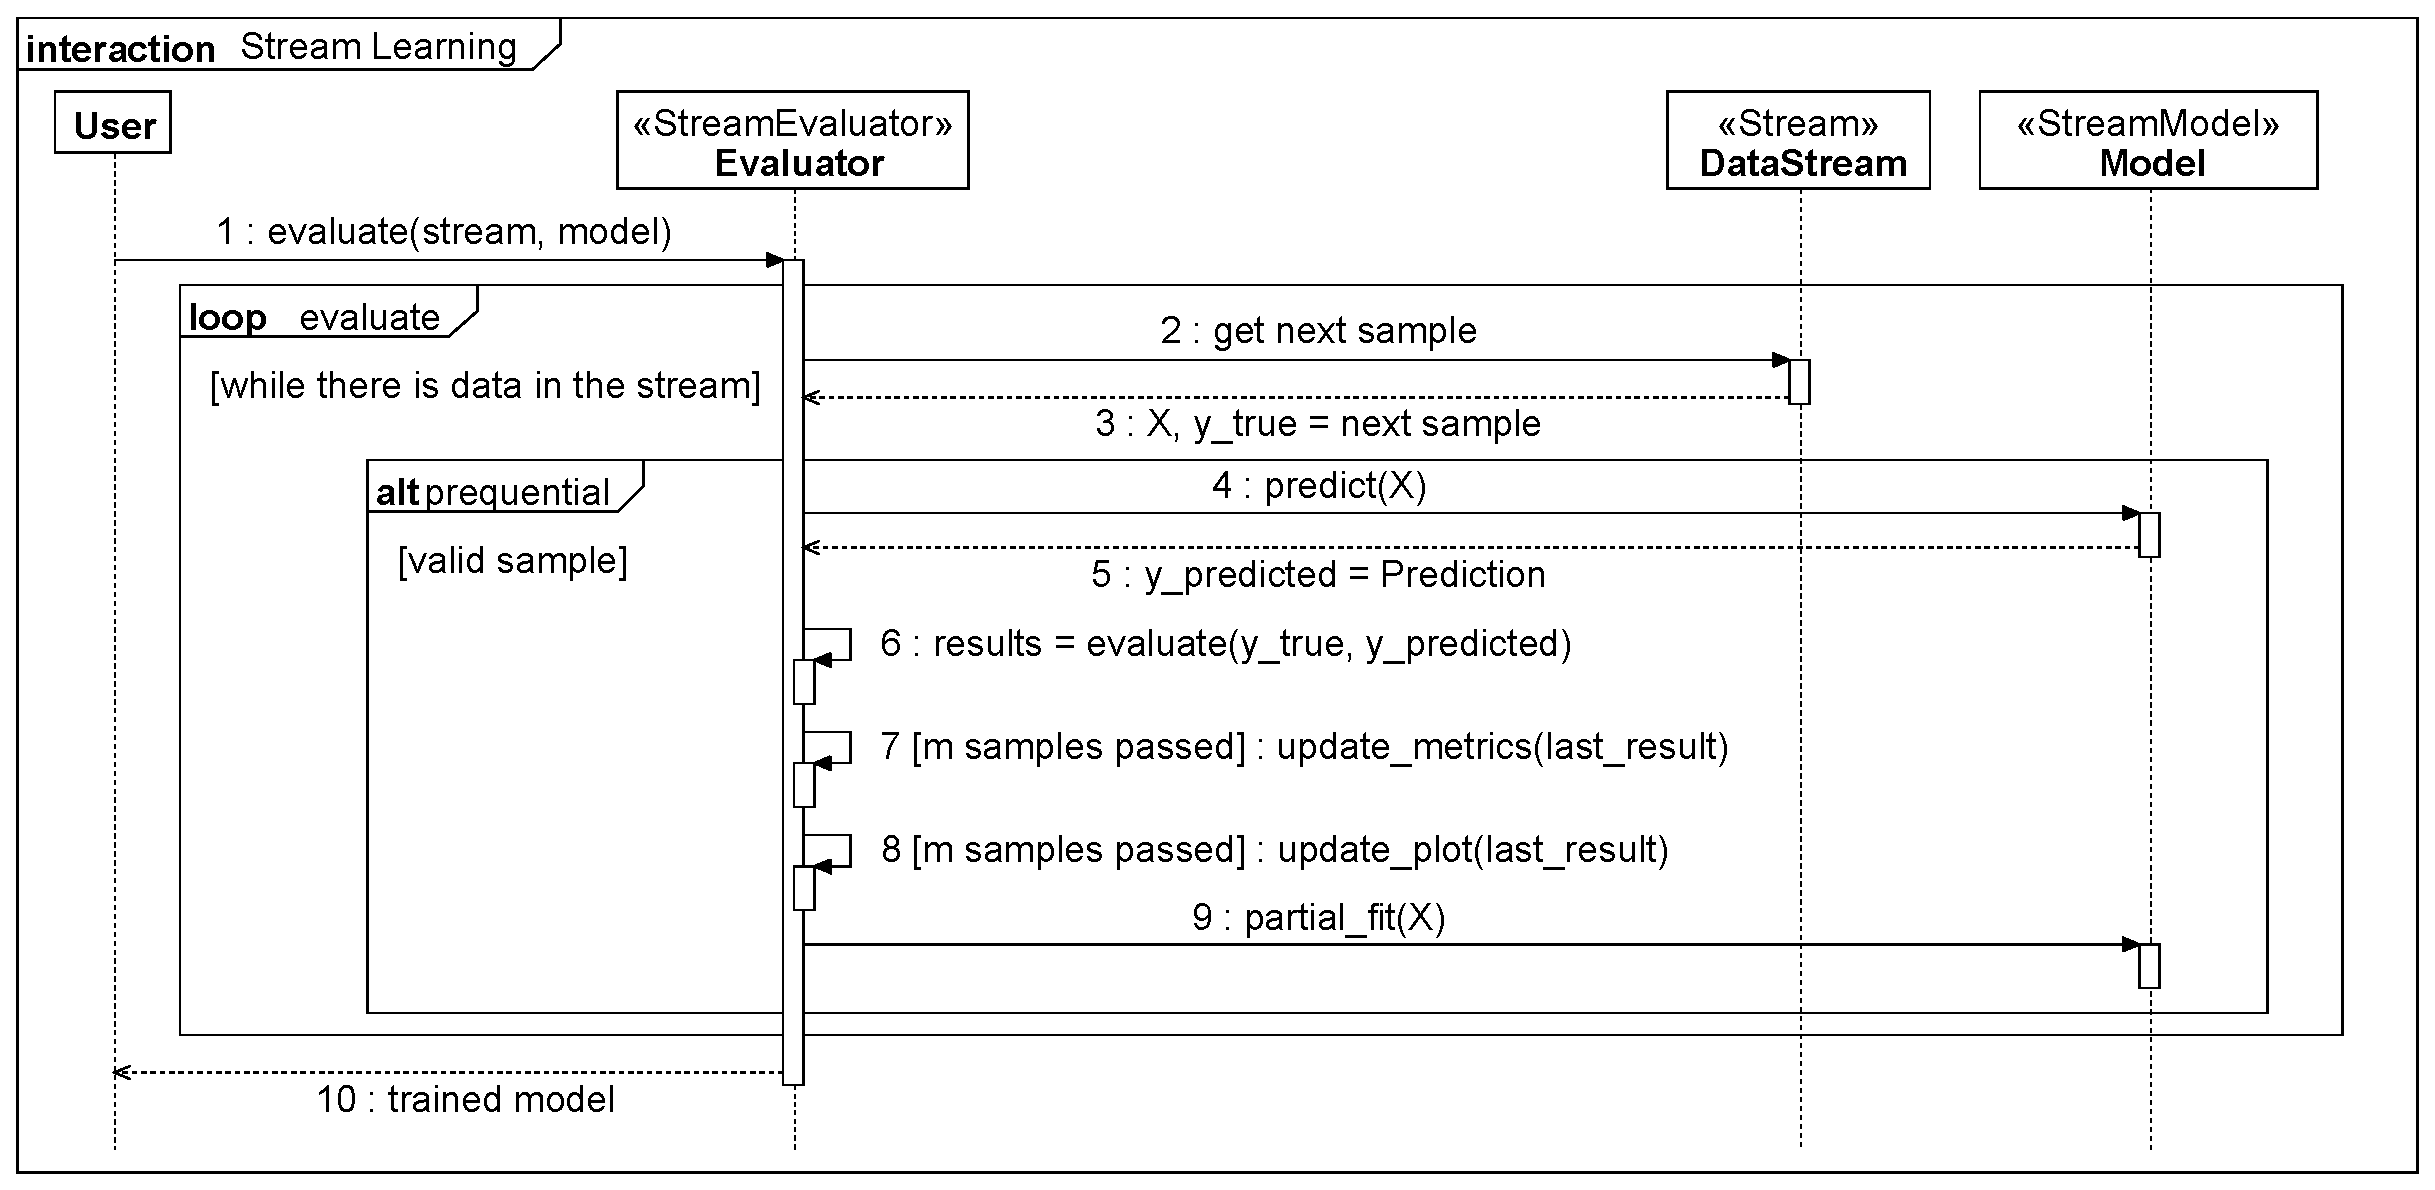
\includegraphics[width=\textwidth]{prequential}
    \caption{Training and testing a stream model using \skmultiflow. This sequence corresponds to prequential evaluation.}\label{fig:learn_seq}
\end{figure}

\section{Development}\label{sec:Development}
The \skmultiflow~package is distributed under the BSD License. Development follows the FOSS principles and encompasses:
\begin{itemize}[noitemsep]
\item A webpage, \url{https://scikit-multiflow.github.io/}, including documentation and user guide. Both, documentation and user guide, are living documents that are continuously updated to reflect the current stage of \skmultiflow.
\item Version control via git. The source code of the package is publicly available on Github at \url{https://github.com/scikit-multiflow/scikit-multiflow}
\item Package deployment and software quality are enforced via continuous integration and functional testing, \url{https://travis-ci.org/scikit-multiflow/scikit-multiflow}
\end{itemize}

% Acknowledgements should go at the end, before appendices and references

% \acks{We would like to acknowledge support for this project
% from the National Science Foundation (NSF grant IIS-9988642)
% and the Multidisciplinary Research Program of the Department
% of Defense (MURI N00014-00-1-0637). }

\bibliography{biblio}

\end{document}